% ============================================================
\chapter*{Prologue: A Linear Game of Life}
\addcontentsline{toc}{chapter}{Prologue: A Linear Game of Life}
\label{ch:prologue}
% ============================================================

\section*{A Game That Started It All}
\addcontentsline{toc}{section}{A Game That Started It All}

Conway's Game of Life is played on a grid of square cells. Each cell is either
alive or dead. Every tick, each cell looks at its eight neighbors and updates
according to a short counting rule. There is no randomness, no geometry beyond
the grid, and no hidden memory.

Even so, small patterns can behave like objects. The famous glider moves
diagonally across the grid, returning to the same shape every four steps, but
shifted by one cell.

\begin{figure}[h]
  \centering
  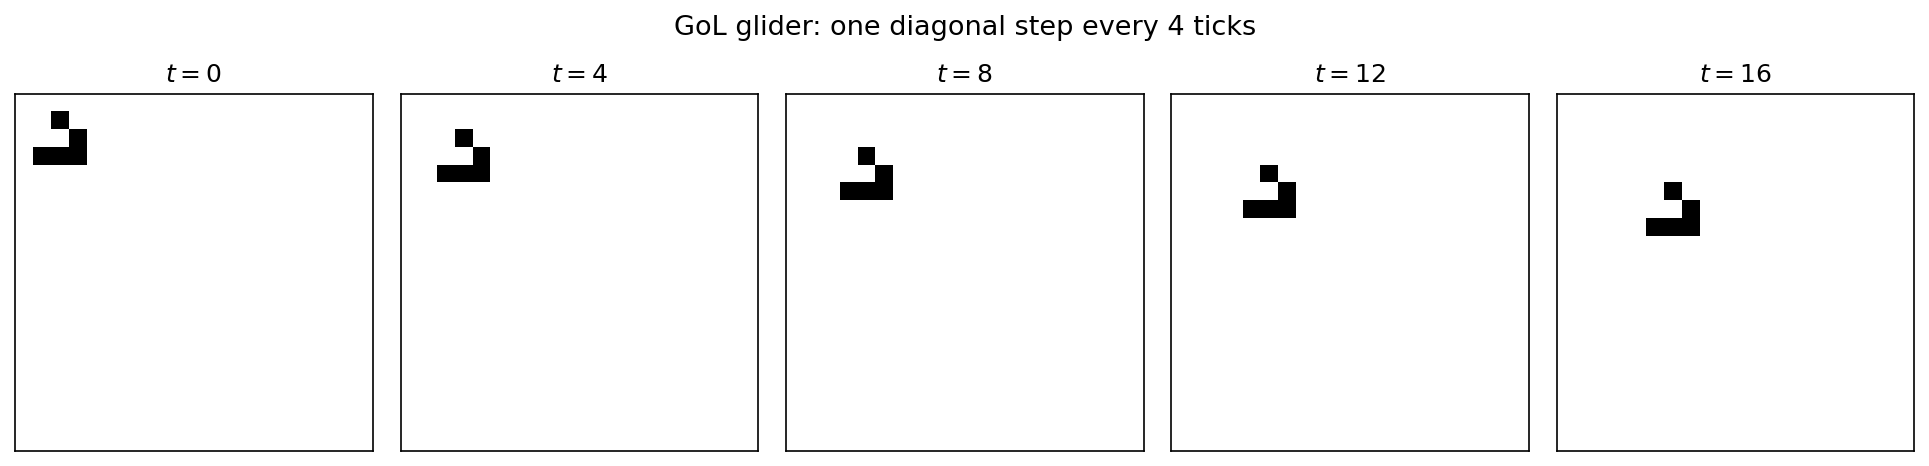
\includegraphics[width=0.92\textwidth]{book/assets/figures/intro/fig_glider.png}
  \caption{A Game-of-Life glider at five snapshots, each four ticks apart.}
\end{figure}

The glider raises a question that will follow us through the book: why does a
pattern stay coherent while a rule repeatedly transforms it? Linear algebra is
one language for answering that kind of question.

\section*{A Linear Version}
\addcontentsline{toc}{section}{A Linear Version}

The Game of Life is nonlinear: it counts neighbors and compares the count to a
threshold. To make the question analyzable, replace alive/dead cells by real
numbers. Let $u_{m,n}(t)$ be the activity at grid cell $(m,n)$ at time $t$, and
define
\[
  u_{m,n}(t+1)
  =
  1.2\,u_{m+1,n+1}(t)+0.8\,u_{m-1,n-1}(t).
\]
This is not the Game of Life. It is a deliberately simplified linear model of
a rule with a preferred diagonal direction.

If the whole grid has $N$ cells, then a state is a vector in $\R^N$. One time
step is a map $T:\R^N\to\R^N$. The rule is linear because
\[
  T(u+v)=T(u)+T(v),
  \qquad
  T(\lambda u)=\lambda T(u).
\]
Those two identities are the price of admission. In exchange, we get a theory
that can predict what the rule does to every possible initial condition.

\section*{Experiments Before Theory}
\addcontentsline{toc}{section}{Experiments Before Theory}

Start with a single active cell. The signal spreads only along the
north-east/south-west diagonal, because the rule only talks to those two
neighbors.

\begin{figure}[h]
  \centering
  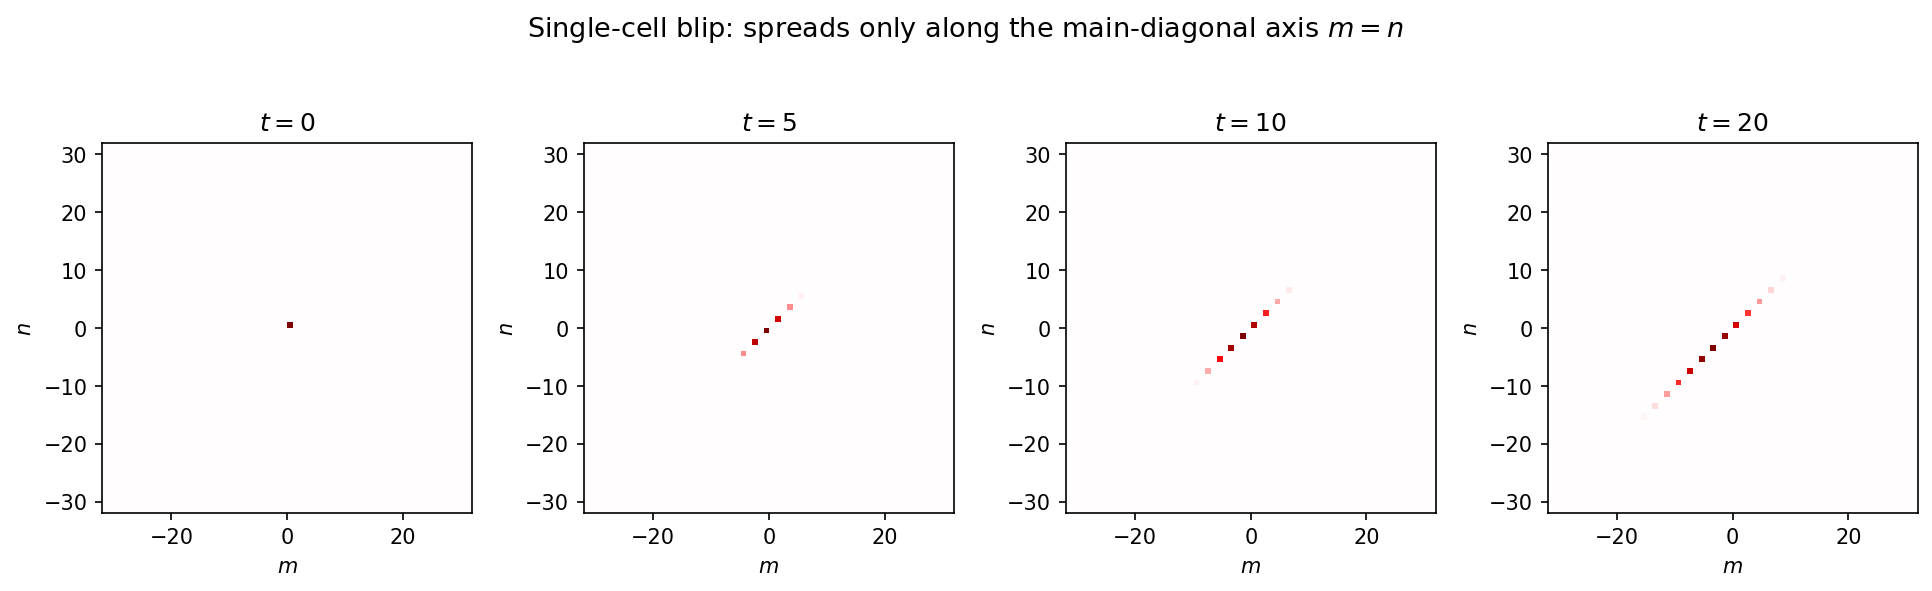
\includegraphics[width=0.92\textwidth]{book/assets/figures/intro/fig_blip.png}
  \caption{A single blip evolved under the linear diagonal rule.}
\end{figure}

Now seed waves along different diagonals. Some patterns grow together; others
decay or break apart because their wavelengths are amplified by different
amounts.

\begin{figure}[h]
  \centering
  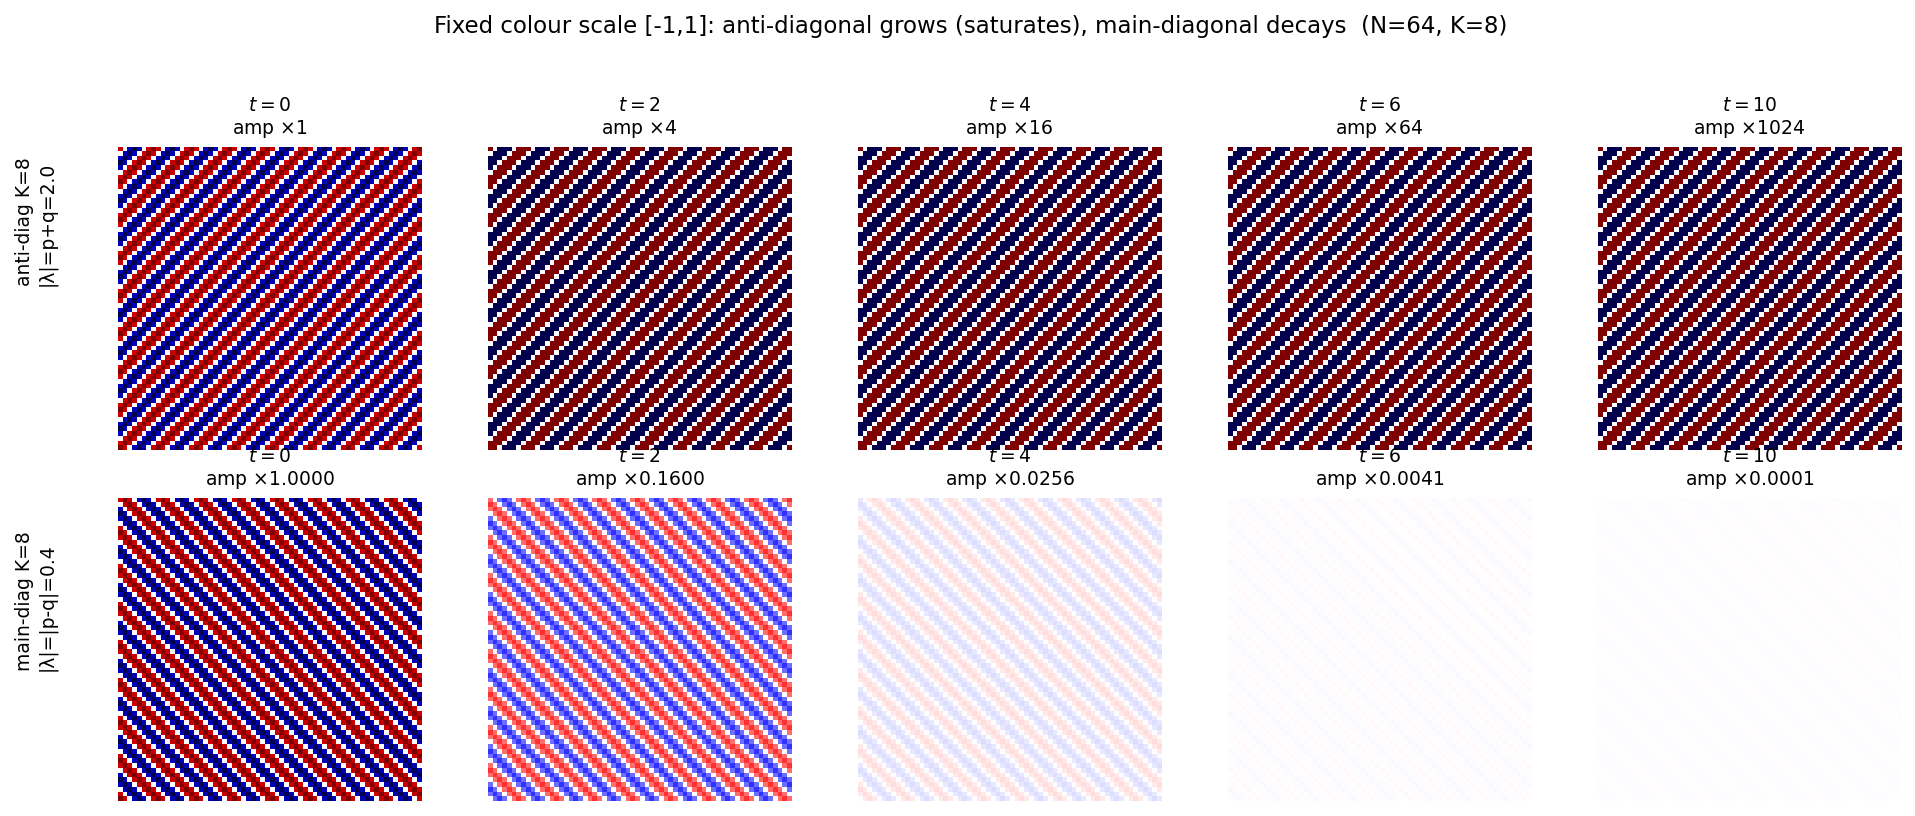
\includegraphics[width=0.92\textwidth]{book/assets/figures/intro/fig_stripes.png}
  \caption{Different diagonal wave patterns can be amplified at different rates.}
\end{figure}

The important lesson is not the particular number $1.2$ or $0.8$. The lesson
is that a rule can have preferred directions. In linear algebra, those
preferred directions are eigenvectors, and the amplification factors are
eigenvalues.

\section*{The Amplification Map}
\addcontentsline{toc}{section}{The Amplification Map}

For a translation-invariant rule, Fourier waves are the natural test patterns.
Each wave is transformed by a simple scaling factor. The following plot shows
the magnitude of that scaling factor for all wave directions in the grid.

\begin{figure}[h]
  \centering
  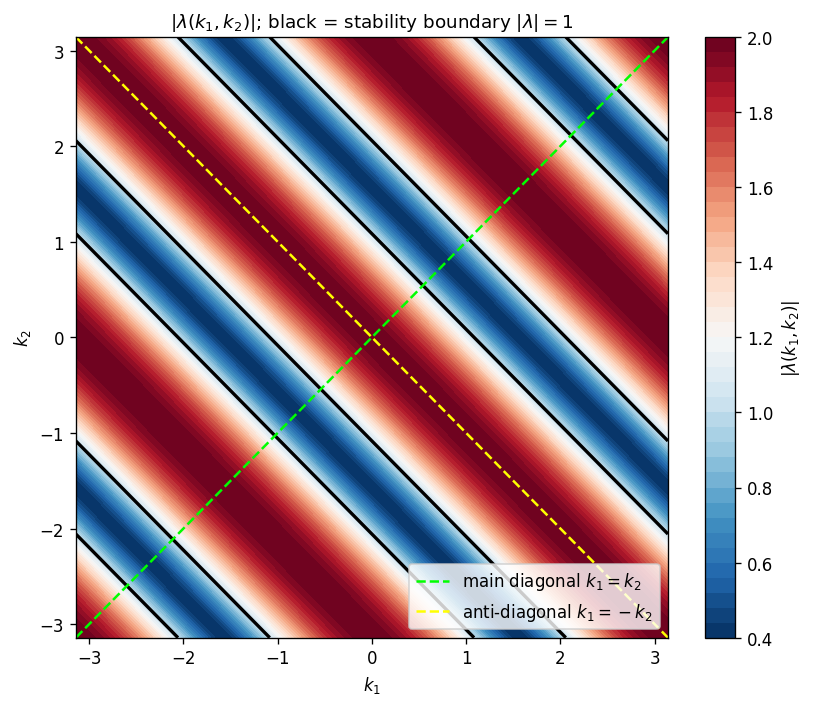
\includegraphics[width=0.72\textwidth]{book/assets/figures/intro/fig_amplification_map.png}
  \caption{Growth rate for Fourier waves under the diagonal linear rule.}
\end{figure}

You are not expected to derive this picture yet. By the end of the book, the
ingredients will be familiar: vector spaces, linear maps, bases, eigenvectors,
the spectral theorem, the SVD, and optional Fourier methods.

\begin{aimlbox}
This example is AI/ML-primed, not AI/ML-specialized. A data set, a signal, an
image, or a model state can be treated as a vector. A linear rule transforms
that vector. A good basis exposes what the rule is really doing.
\end{aimlbox}

\section*{The Course Promise}
\addcontentsline{toc}{section}{The Course Promise}

The point of this book is not to make every problem linear. Most real systems
are nonlinear. But linear structure is the part we can compute with, prove
things about, approximate with, and use inside larger algorithms. Neural
networks, regression, image filters, recommender systems, and scientific
models all rely on linear algebra as one of their basic layers.

\section*{Prologue Summary}
\addcontentsline{toc}{section}{Prologue Summary}

\begin{itemize}
  \item A state with finitely many numbers can be treated as a vector.
  \item A linear rule preserves addition and scalar multiplication.
  \item Eigenvectors are patterns whose direction is preserved by a rule.
  \item A good basis can turn a complicated rule into a simple one.
\end{itemize}

\section*{Where This Appears Later}
\addcontentsline{toc}{section}{Where This Appears Later}

Linear maps begin in Chapter~\ref{ch:matrices-linear-maps}. Eigenvectors and
dynamics appear in Chapter~\ref{ch:eigenvalues-dynamics}. Convolution and the
discrete Fourier transform return in Chapter~\ref{ch:images-convolution-dft}.

\input{book/exercises/prologue-exercises}
